\section{Technical Solution}

As mentioned in the design challenges section, many parts of the solution are flexible and can withstand change. Some concepts has to be consistent and must be respected. Such a concept is the communication protocols. 

\subsection{Protocols}

Since the interactions happen between separate devices, defined protocols are used to make sure the information is handled correctly. 

\subsubsection{Sending current client information to the server}
At regular intervals, the client program is responsible for supplying fresh data to the server as mentioned in the 'Roles and Responsibilities' section. This is done through UDP packets being sent to the server. Since these packets are sent from every user at regular intervals, they will become a substantial part of the server load, as illustrated in figure \ref{fig:udp_packets}. The protocol chosen is therefore the 'maybe' protocol, as it is not urgent that every position update is received server-side. 

\begin{figure}[H]
    \centering
    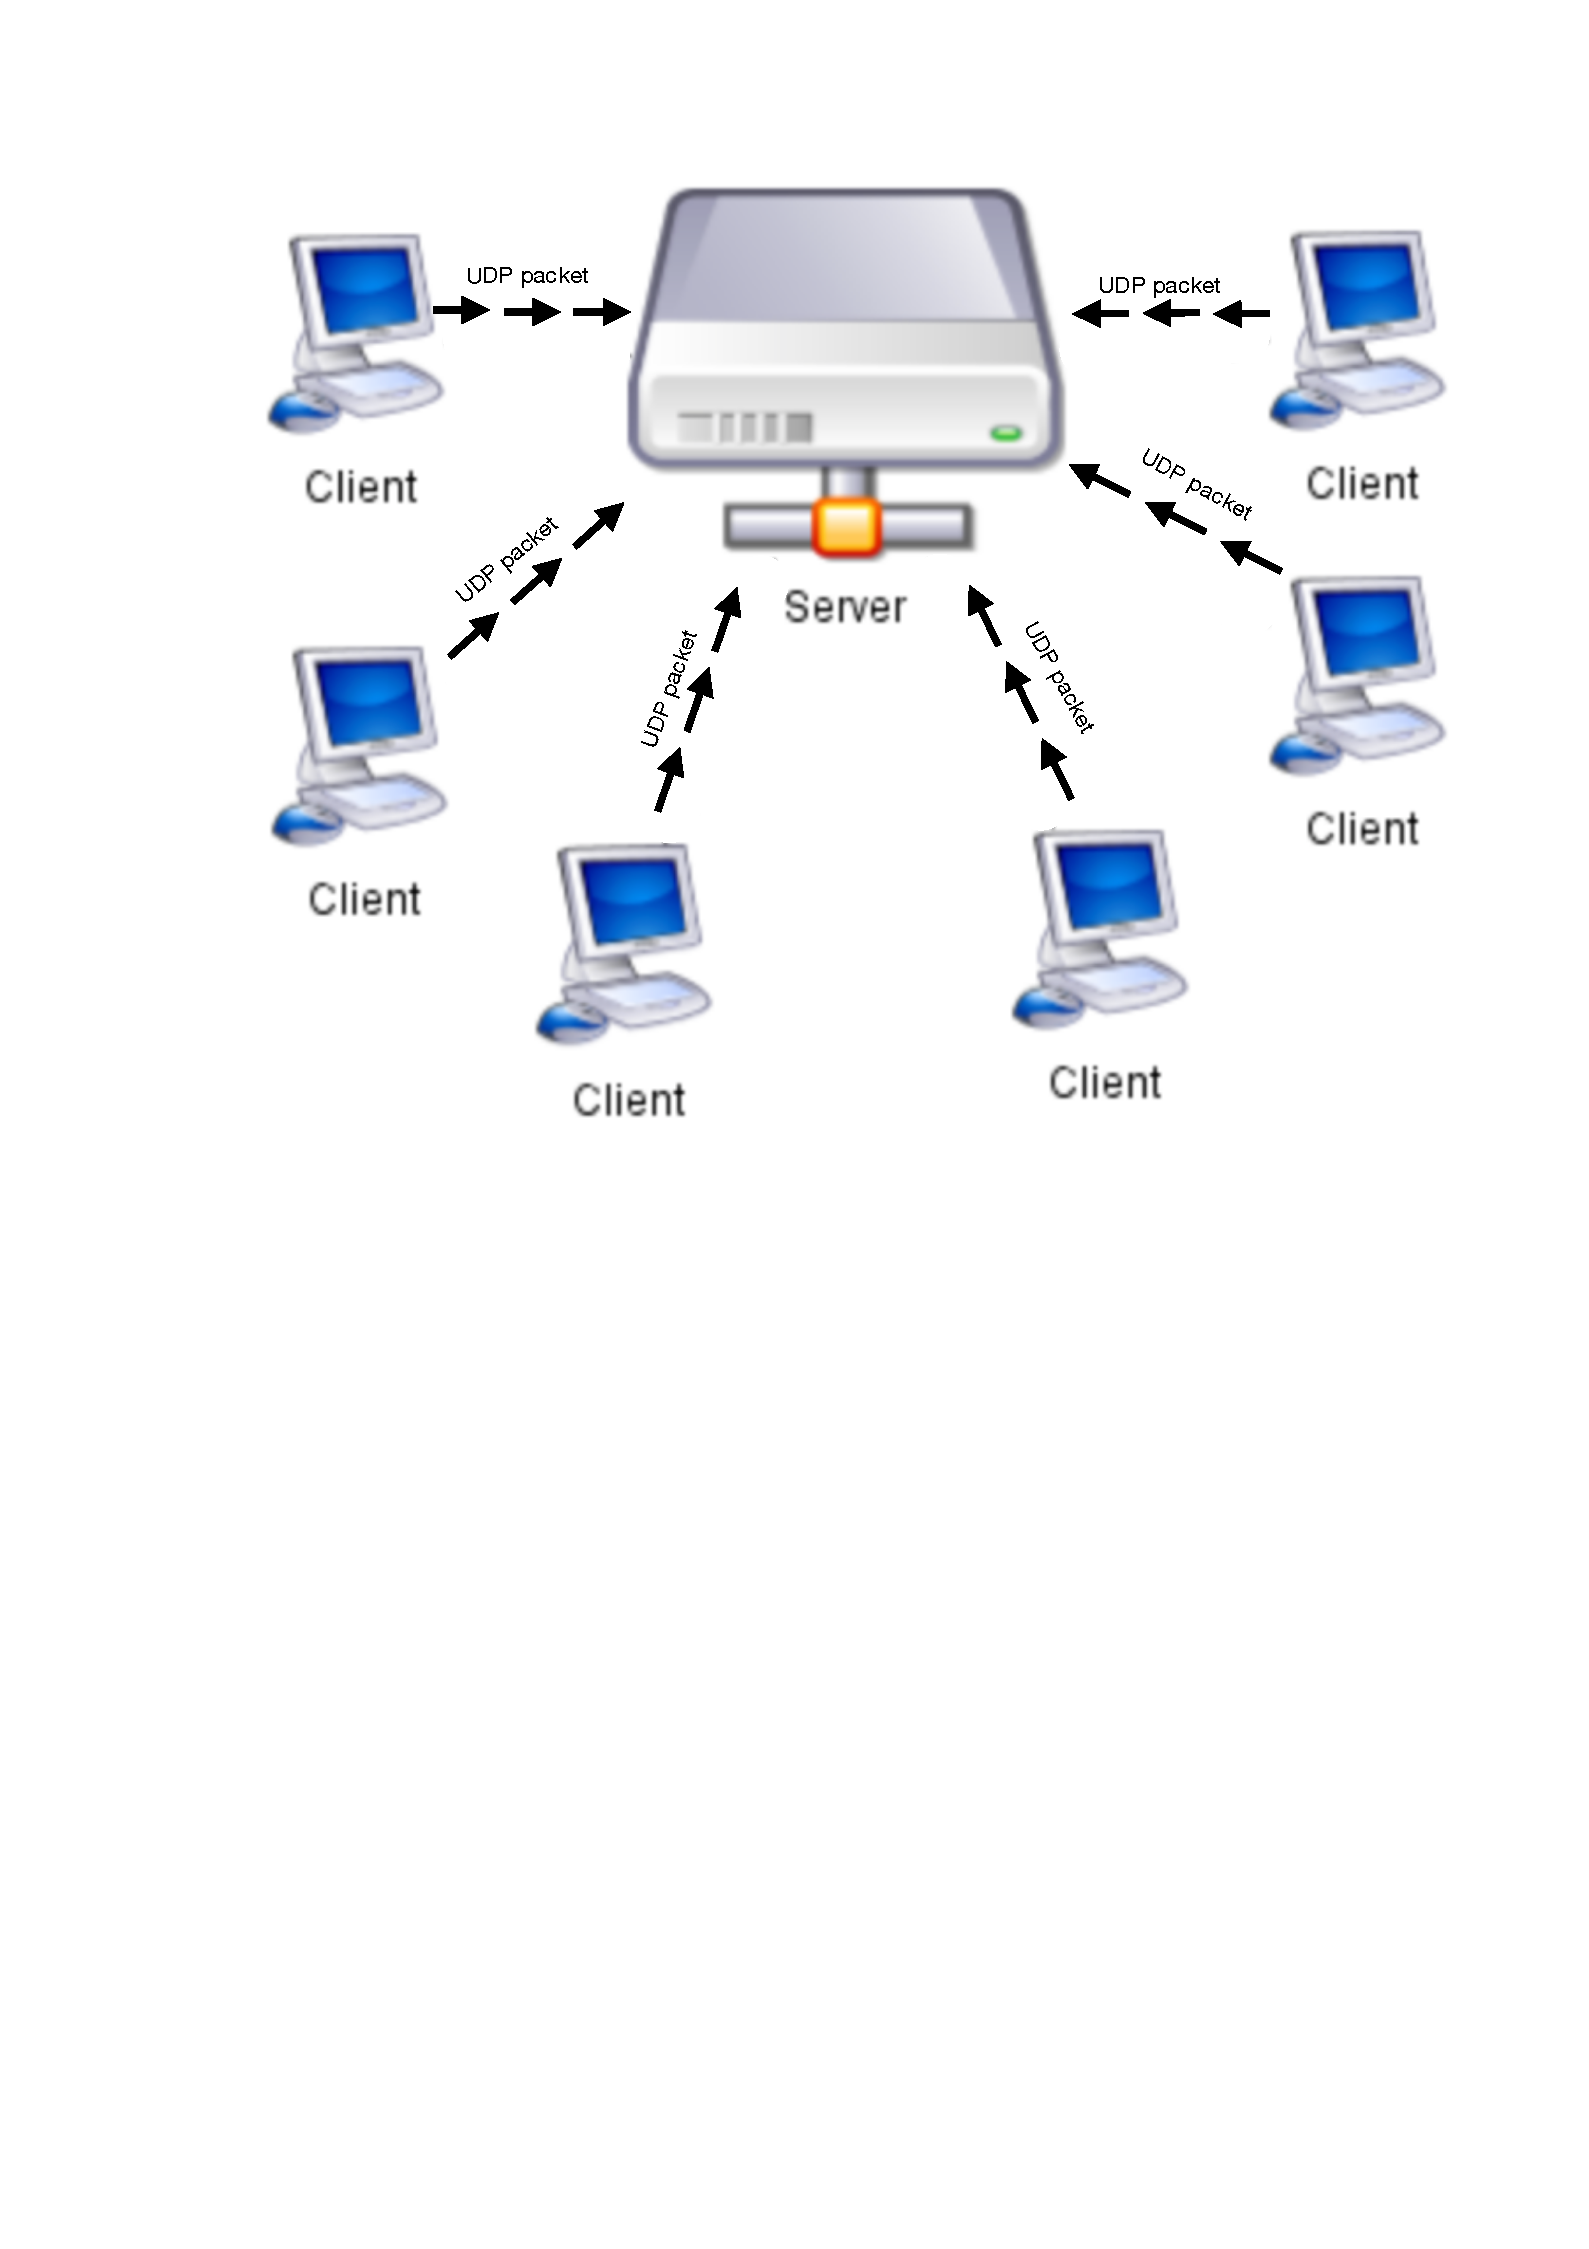
\includegraphics[width=0.6\linewidth]{images/UDPPackets.pdf}
    \caption{UDP packets sent from all clients to server.}
    \label{fig:udp_packets}
\end{figure}

\subsubsection{Requesting heat map}
For the client to retrieve data from the server, it needs to inform the server, that it is active. If the server sent data to all registered clients, bandwidth and computation time would be used on many possibly redundant/non-profitable tasks. For that reason clients perform remote method invocations (RMI) to the server, to gain access to the last computed heat map on the server. For this not to be a bottleneck, the heat map is cropped to a suitable map (based on a specific radius from the user). This way, the complete world density heat map is not sent, but only a small fraction of it.

In case the system suffers from server error or network delay, a timeout time limit is applied to the RMI call. With the same reasoning as the UDP packets, the heat map will not change drastically, and the consequence of a missed heat map will be minor visual effects for the client.


\subsubsection{Getting information from clients in a private group}

As mentioned earlier, client-to-client communication will use the multicast protocol, to prompt the other active users for their information. The sent message will contain the information about the sender, used by the receiving clients to return their position. Once the initial prompt is sent to all connected users\footnote{Clients in the private group, added to the multicast group.}, that client will wait for UDP packets for a preset time period. The returned packets inform the client which other clients are active from the private group.

For this reason, the client application needs two threads. One thread responsible for listening and reacting to other clients prompts, and a second thread responsible for the remaining tasks in order to prevent two clients both waiting for each others response.

The sequence of packets are seen in figure \ref{fig:privateGroupMulticast}.

\begin{figure}[H]
    \centering
    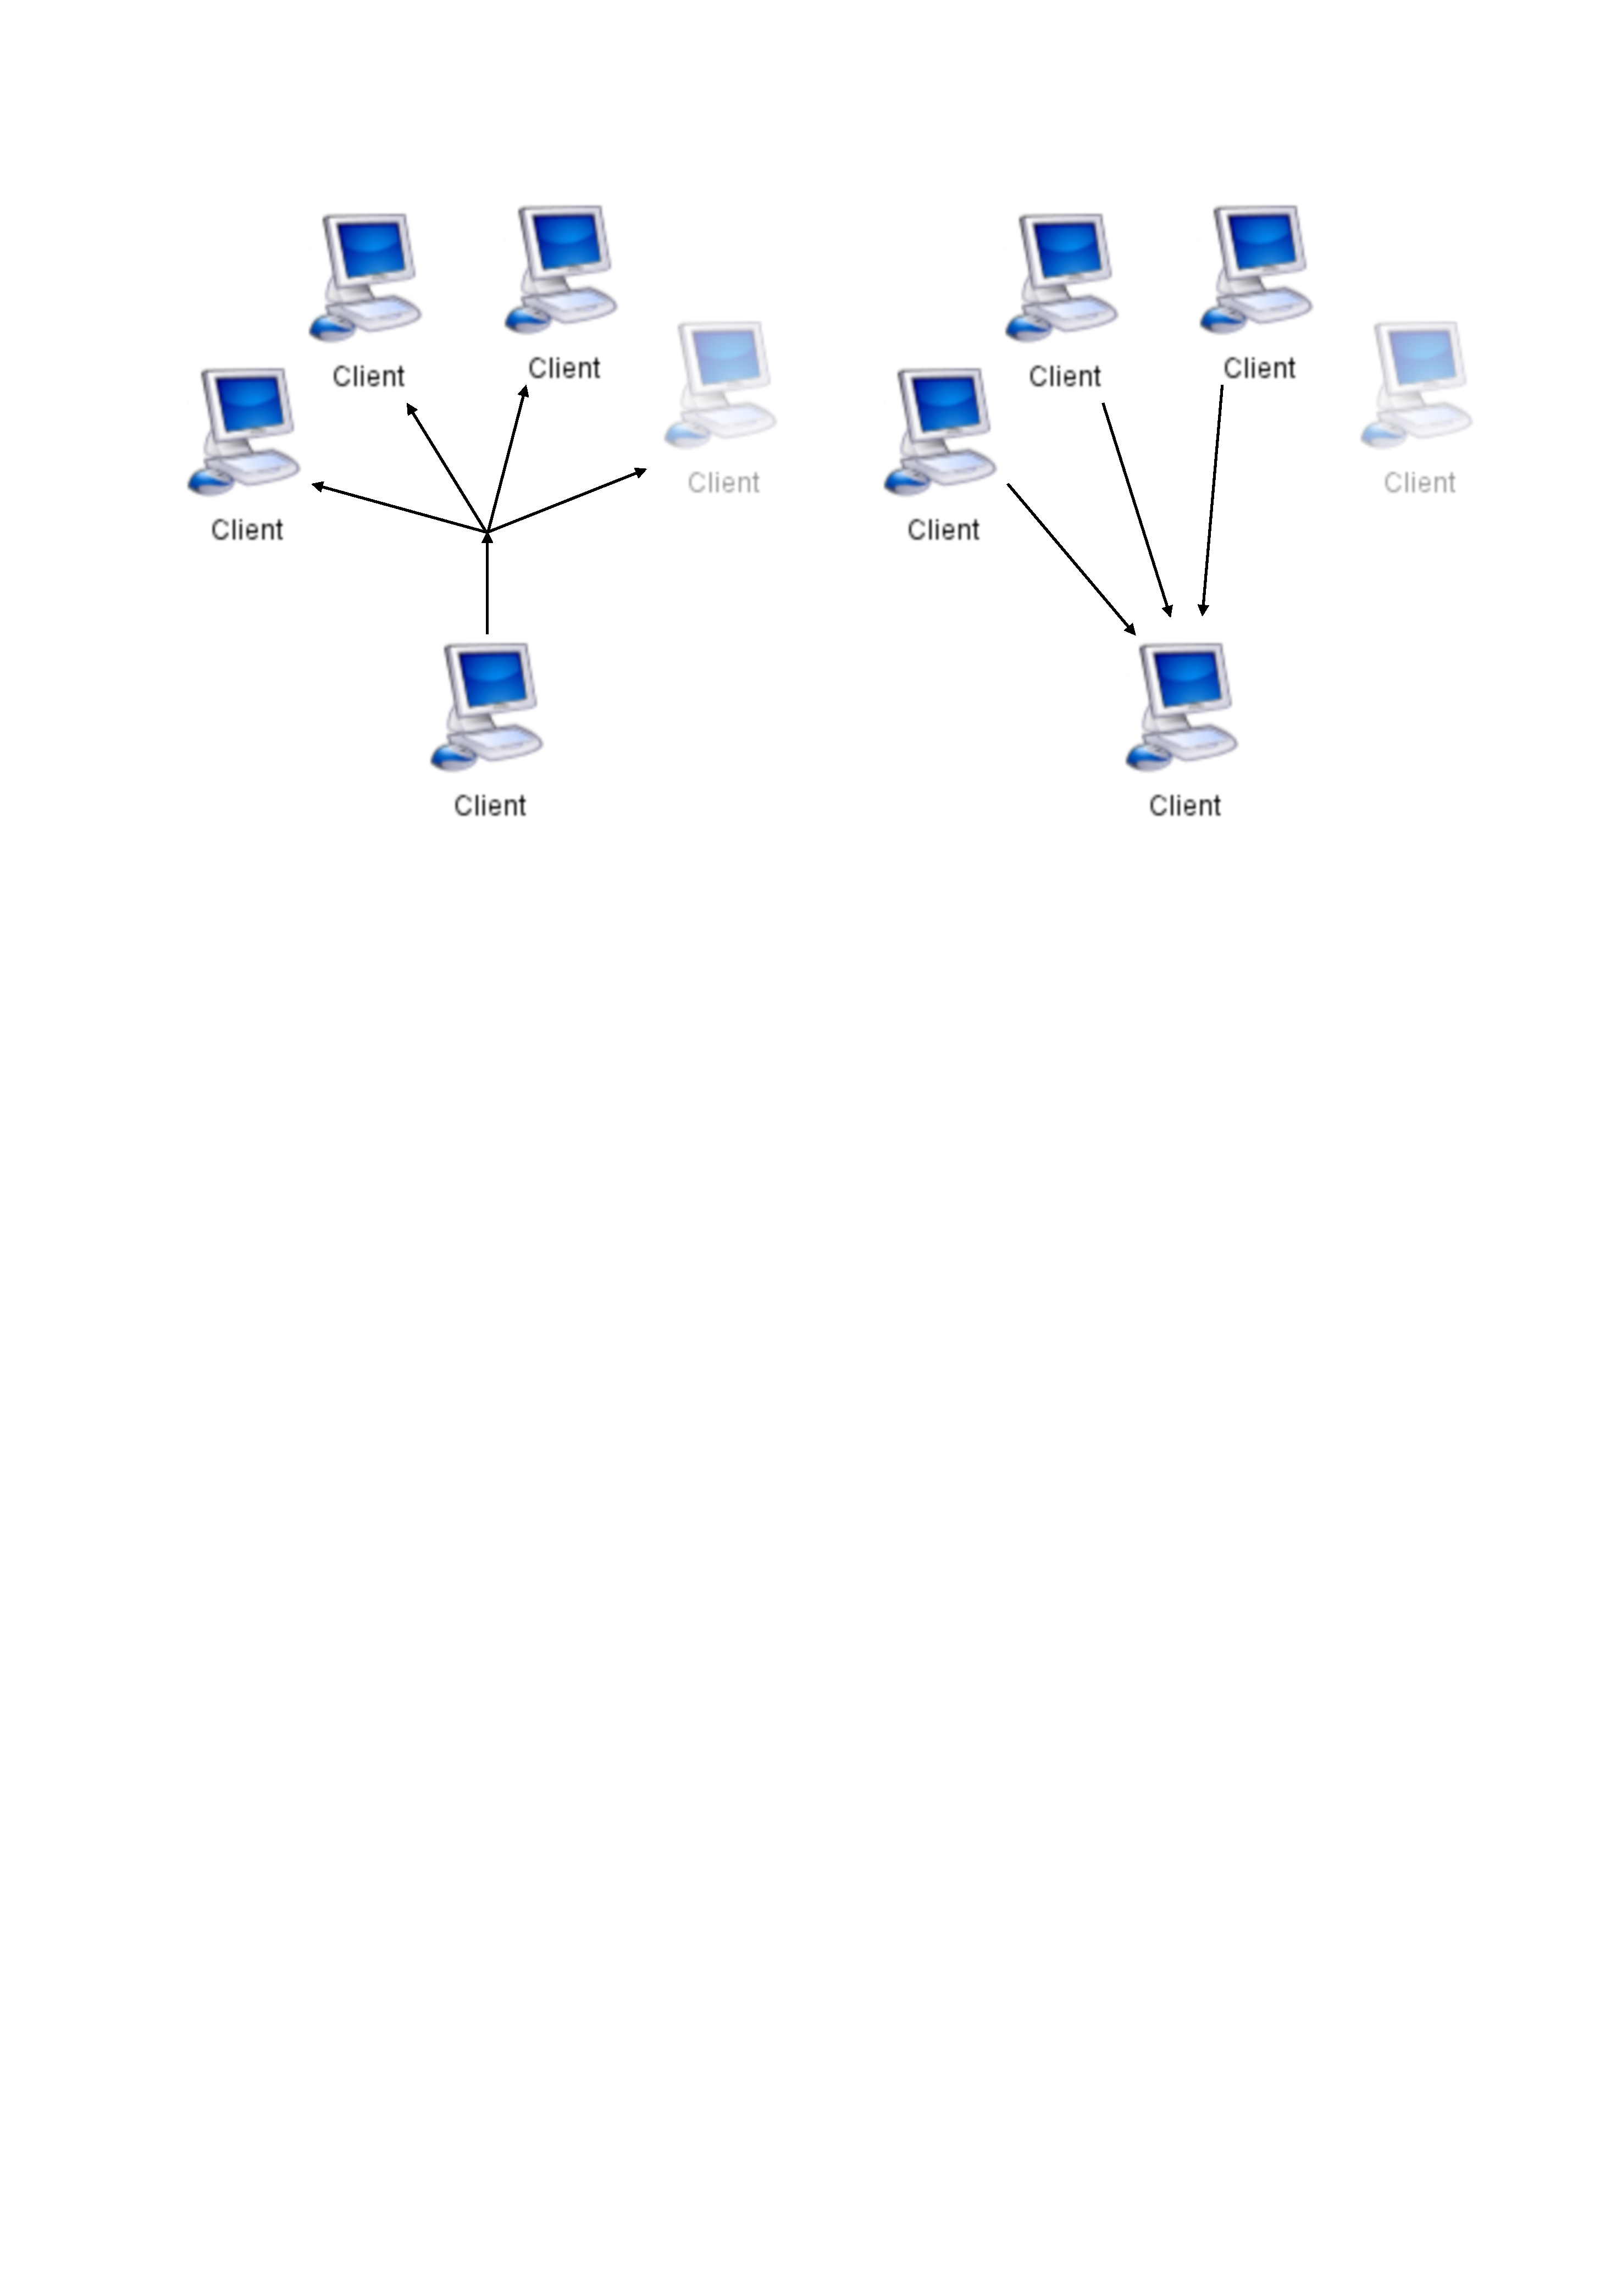
\includegraphics[width=0.9\linewidth]{images/Multicast_client-to-client.pdf}
    \caption{Client requesting information from associates in a private group. The requesting client sees 3 (out of 4) active users in the group after the packet exchange.}
    \label{fig:privateGroupMulticast}
\end{figure}

To heighten security, it is suggested that the packets contain a encrypted key in order to verify that the packet sender is valid and not a con.

\subsubsection{Establishing connection to another client}

In order for clients to be in a the same private group, one client has to send a request to the other client. The client can send queries to the server through RMI calls, to gain a list of clients matching the query, who is not already connected. When the client chooses a client from the list, to send a request to, the request is sent to the server, and stored for the chosen client, which can be retrieved at next update. 

It is not necessary, that the client which the request is sent to, is active, meaning the request has to be stored on the server. When the request is sent to the server, the protocol is 'at least once'. It is necessary that the request is retrieved by the server, and multiple requests can be sent in a map, guaranteeing multiple requests are overwritten.


\subsubsection{Authentication}

Client authentication, both when registering as a new user, and when logging in to their account will be performed using the Facebook API as mentioned in \secref{sec:authencticationChallenge}. Therefore the protocol will use RMI with a specified timeout time limit. 


% Maybe, Atmost-once, Exactly-once, 
% by RMI or message passing
% UDP or TCP




% De provider API's som vi kan bruge.
% https://developers.facebook.com/products/account-creation